\section{Мета роботи}
Отримання навичок у підборі датчиків для захисту приміщень.


\section{Хід роботи}
\begin{itemize}
  \item Скласти опис об'єкта
  \item Скласти список дій, які може зробити передбачуваний порушник
  \item Освоїти методику установки датчиків руху і запропонувати варіант установки датчиків для запропонованих приміщень. Датчики відзначати таким символом, при розміщенні датчиків, враховувати діаграму спрямованості.
  \item Обгрунтувати розміщення кожного датчика.
  \item На кожен тип використовуваних датчиків повинно бути опис технічних характеристик і обгрунтування чому вибрали саме його.
\end{itemize}

Маємо наступний план приміщення згідно варіанту

\begin{figure}[h!]
  \centering
  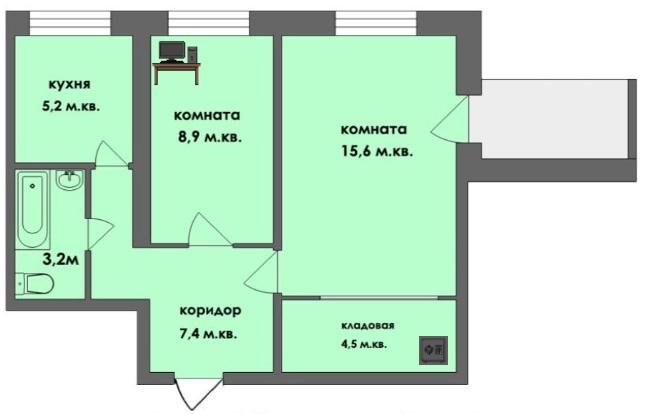
\includegraphics[width=17cm]{reports/info-protection/lab1/assets/flat.jpeg}
\end{figure}

\newpage
Після дослідження приміщення, маємо двокімнатну квартиру:

\begin{itemize}
  \item одна кімната на 15.6 м.кв
  \item одна кімната на 8.9 м.кв
  \item кухня на 5.2 м.кв
  \item кладова на 4.5 м.кв
  \item коридор на 7.5 м.кв
  \item туалет на 3.2 м.кв
\end{itemize}

\textbf{Клієнт хоче зробити розміщення оптимальним відносно ціни та якості}. Людина має ціль захистити свої речі (ПК та сейф) від потрапляння їх до рук зловмисників. Замовник є звичайною людиною яка працює у сфері медецини та просто хоче забезпечити смарт-захист своєї квартири.\\

Потенційно порушник може потрапити до квартири через вхідні двері тамбуру або коридору, а також через вікна, що розташовані у кухні та двох кімнатах.\\

Потенційними предметами зацікавленості загарбника є комп`ютер та сейф. З ціллю безпеки сейф розташовано у кладовій.\\

Виходячи з вище описаного та показаного я пропоную купити один датчик 360 градусів але дуже хороший та розмістити у центрі квартири, оскільки несучі стіни не дуже товсті, а перегоридки між кімнатами тонкі то одного \href{https://www.svit-lamp.ua/datchik-rukhu-mikrokhvilovij-360-230v-bilij/?srsltid=AfmBOorw4jHdgdEdof7Mnl2rhz5X9qELiKz2BF_z3zYOYPQeU4Vz-uxE}{датчика руху мікрохвильовий 360°} вистачить з головою. \\

Також не будемо забувати що НВЧ датчики є шкідливими для людини тому чим менше їх буде у нашому випадку тим краще, бо приміщення не є складським та в ньому буде жити людина (можливо з тваринами). В такому випадку треба розташувати датчик максимально в центрі квартири та у кімнаті де не буде часто знаходитися людина та інші живі істоти. Тому треба порекомендувати перенести комп`ютер ц іншу кімнату якщо це можливо.

\newpage
Датчик приведений у посиланні має основні ключові характеристики для нас:
\begin{itemize}
  \item Захист IP20 - тільки для використання всередині приміщень.
  \item Кут виявлення: 360°.
  \item Дальність дії датчика: 2-16 м (регулюється).
\end{itemize}

Це лише основне що нас більш цікавить, також є інші корисні налаштування.

Вибір саме цього типу датчиків обумовлений їх зарекомендованою якістю та ргульованою дистанцією спрацювання, що є дуже гарним для велокої квартири. Виходячи з цього я пропоную наступне розміщення датчику та поставити радіус дії 8-12 метрів щоб охопити балкон та кладову та не сканувати зайві області сусідніх квартир:

\begin{figure}[h!]
  \centering
  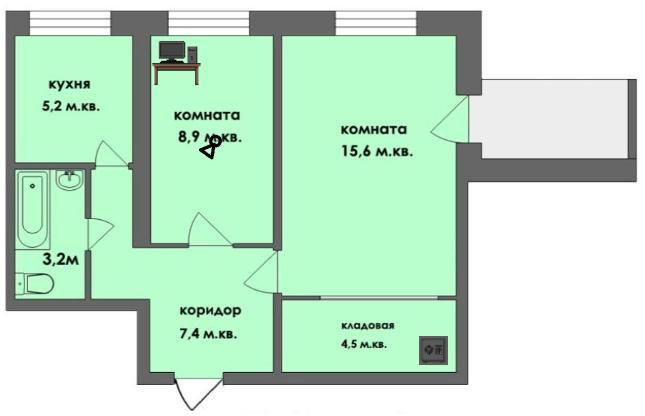
\includegraphics[width=17cm]{reports/info-protection/lab1/assets/flat-filled.jpeg}
\end{figure}

\section{Висновок}
У підсумку я виконав поставлену задачу та встановив у квартирі недорогий та хороший датчик вартістю 879 грн, що є оптимальною ціною для замовника. Також мінімізував загрозу здоров'ю людини через розміщення лише одного датчика у квартирі.
